The flow of data through the system is most critical during the creation of a new recommender agent. This process transforms raw user-uploaded files into a structured, multi-faceted data asset that powers the agent's conversational and recommendation capabilities. The end-to-end data flow for this process is illustrated in the flowchart in Figure~\ref{FIG:DATA_FLOWCHART}.

\begin{figure}[Data Flowchart for Agent Creation]{FIG:DATA_FLOWCHART}{Data Flowchart for the Agent Creation process.}
    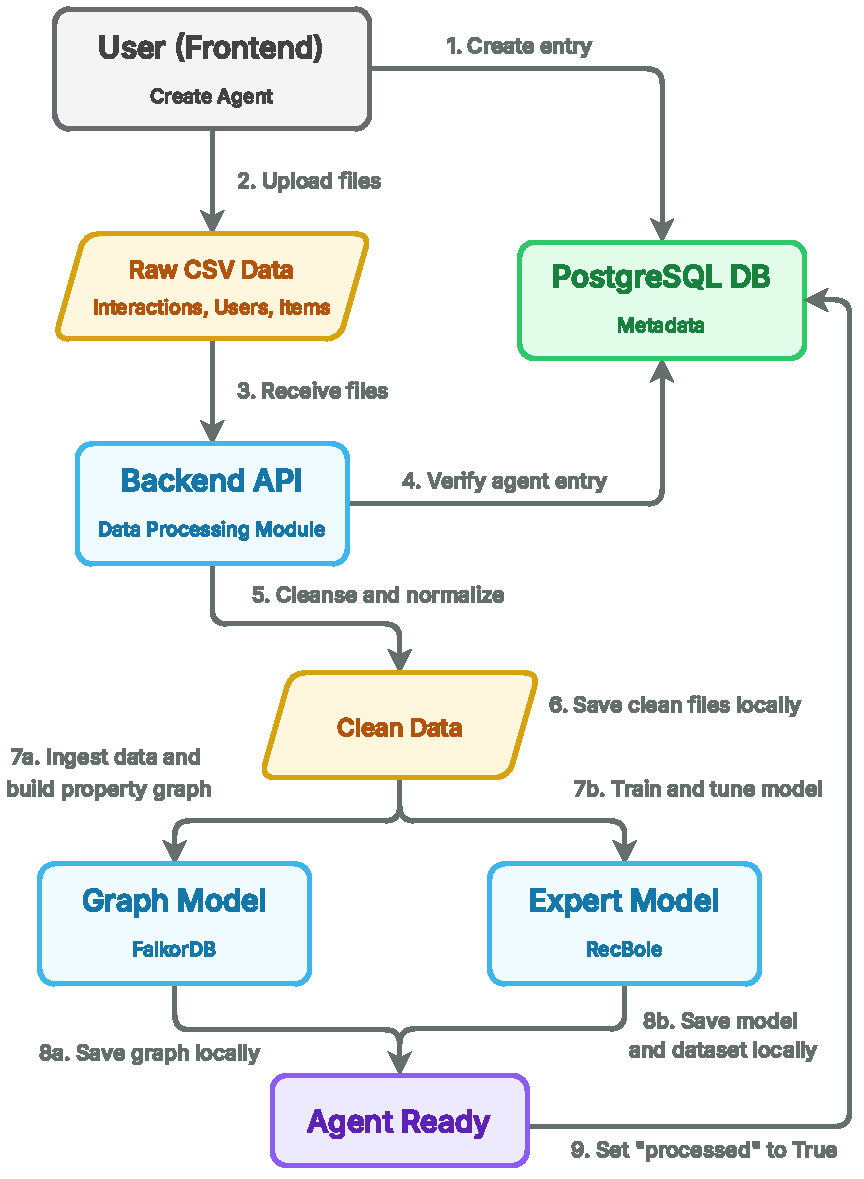
\includegraphics[width=0.785\textwidth]{data_flowchart.pdf}
\end{figure}

The process can be summarized in the following steps:
\begin{compactenum}
    \item An entry is created in the \texttt{RecommenderAgent} table in the PostgreSQL database, and a corresponding row is inserted in the \texttt{RecommenderAgentVisibility} table through a trigger, to manage its real-time visibility on the frontend.
    \item The user uploads raw CSV files (interactions, items, users) and column configuration via the frontend interface.
    \item The backend \acs{api} receives the files and checks the existence of the agent metadata. If the entry exists, it stores the files temporarily.
    \item The Data Processing Module initiates its pipeline, performing data cleansing and normalization. Afterwards, each file is persisted in a local, unique directory.
    \item The cleaned data is then used in two procedures:
    \begin{compactenum}
        \item The FalkorDB recommender component ingests the user-item interaction data, building a property graph and computing graph metrics like PageRank.
        \item An expert model \cite{EASER} is trained through RecBole on the cleaned data, and the resulting model and dataset artifacts are saved.
    \end{compactenum}
    \item Upon successful completion of both procedures, the agent's \texttt{processed} flag is switched to \texttt{True} in the PostgreSQL database, making the agent available on the platform.
\end{compactenum}
